\section{Task 2: Regression -- Modelling the Relationship between Server Metrics}
\label{sec:task2}

\subsection{Task 2.1: Least squares parameter estimates}
For each model a design matrix was built from the transformed inputs plus a column of ones, and Equation~\eqref{eq:ls} was solved with \texttt{solve(t(X) \%*\% X) \%*\% t(X) \%*\% y} using all 10{,}000 samples (Appendix~\ref{app:task2}, section ``Task 2.1''). As a check, Model~1 was also fitted with \texttt{lm()}, which gave the same estimates to every printed digit. Table~\ref{tab:theta} lists the results.

\begin{table}[H]
\centering
\caption{Least squares estimates $\hat{\boldsymbol\theta}$ for the five candidate models (all data).}
\label{tab:theta}
\begin{tabular}{lll}
\toprule
Model & Term & Estimate \\
\midrule
1 & $x_4$ / $x_1^2$ / $x_1^3$ & 3.0940 / $-4.0550$ / 2.3840 \\
  & $x_2^4$ / $x_1^4$ / bias & $-0.005608$ / $-0.09913$ / 930.83 \\
\midrule
2 & $x_4$ / $x_1^3$ / $x_3^4$ & 4.4805 / 1.20018 / 0.800003 \\
  & bias & 120.022 \\
\midrule
3 & $x_3^3$ / $x_3^4$ / bias & $-0.03076$ / 0.80153 / 308.585 \\
\midrule
4 & $x_2$ / $x_1^3$ / $x_3^4$ & 0.1170 / 1.20032 / 0.79994 \\
  & bias & 132.854 \\
\midrule
5 & $x_4$ / $x_1^2$ / $x_1^3$ & 4.4805 / $-0.01019$ / 1.20146 \\
  & $x_3^4$ / bias & 0.800003 / 120.083 \\
\bottomrule
\end{tabular}
\end{table}

The estimates already show a pattern. Every model that contains $x_3^4$ estimates its coefficient as about 0.80, and every model that contains $x_1^3$ estimates about 1.20. Models~2 and~5 give almost the same values for every shared term ($x_4\approx4.48$, bias $\approx120$), and the extra $x_1^2$ term in Model~5 is close to zero ($-0.010$). Model~1 has no $x_3$ term at all, so its intercept (930.8) is pulled towards the mean of $y$ to make up for it.

\subsection{Task 2.2: Residual sum of squares}
The RSS of each model (Appendix~\ref{app:task2}, ``Task 2.2'') is given in Table~\ref{tab:crit}. The RSS values differ by more than four orders of magnitude. Models~2 and~5 have by far the lowest RSS (about $2.51\times10^5$). The models without the right terms are much worse: Model~4 swaps $x_4$ for $x_2$ ($2.06\times10^6$), Model~3 has no CPU or network term ($3.05\times10^8$), and Model~1 has no disk term ($7.54\times10^9$). This agrees with Task~1, where $x_3$ was found to be the main driver of power.

\subsection{Task 2.3: Log-likelihood}
The variance $\hat\sigma^2=\text{RSS}/(n-1)$ and the log-likelihood from Equation~\eqref{eq:loglik} were computed for each model. For Models~2 and~5, $\hat\sigma^2\approx25.08$, so the noise standard deviation is about 5.0\,W. This is very small next to the spread of $y$ (884\,W), and suggests that these models capture almost all of the signal. Because $\hat\sigma^2$ is proportional to the RSS, the log-likelihood ranks the models in the same order as the RSS.

\subsection{Task 2.4: AIC and BIC}
AIC and BIC were computed from Equation~\eqref{eq:aicbic} with $k$ equal to the number of columns of each design matrix, including the bias. Table~\ref{tab:crit} collects all the criteria. $\Delta$AIC and $\Delta$BIC show the difference from the best model.

\begin{table}[H]
\centering
\caption{Model comparison criteria ($n=10{,}000$). The lowest AIC and BIC (selected model) are in bold.}
\label{tab:crit}
\small
\setlength{\tabcolsep}{4pt}
\begin{tabular}{crrrrrrrr}
\toprule
Model & $k$ & RSS & $\hat\sigma^2$ & $\ln p(D|\hat\theta)$ & AIC & BIC & $\Delta$AIC & $\Delta$BIC \\
\midrule
1 & 6 & $7.538\times10^{9}$ & 753871.8 & $-81853.8$ & 163719.6 & 163762.8 & 103111.7 & 103126.1 \\
2 & 4 & $2.508\times10^{5}$ & 25.08 & $-30300.0$ & \textbf{60607.9} & \textbf{60636.7} & \textbf{0.0} & \textbf{0.0} \\
3 & 3 & $3.048\times10^{8}$ & 30478.8 & $-65812.8$ & 131631.7 & 131653.3 & 71023.8 & 71016.5 \\
4 & 4 & $2.056\times10^{6}$ & 205.65 & $-40819.7$ & 81647.5 & 81676.3 & 21039.6 & 21039.6 \\
5 & 5 & $2.508\times10^{5}$ & 25.08 & $-30299.8$ & 60609.6 & 60645.6 & 1.7 & 8.9 \\
\bottomrule
\end{tabular}
\end{table}

Model~2 has the lowest AIC (60607.9) and the lowest BIC (60636.7). Model~5 comes a close second. Its RSS is only 8.3 lower than that of Model~2 ($250802.2$ against $250810.5$), which raises its log-likelihood by just 0.17. That is far too little to pay for the extra parameter, so its AIC is 1.67 higher and its BIC 8.88 higher. Models~1, 3 and~4 are worse by tens of thousands of units and can be ruled out.

\subsection{Task 2.5: Distribution of the residuals}
Figure~\ref{fig:res} shows a histogram and a normal Q-Q plot of the residuals of each model (Appendix~\ref{app:task2}, ``Task 2.5''). Since the noise in the data is Gaussian, the correct model should leave residuals that are Gaussian too.
\begin{itemize}
  \item \textbf{Model 1}: the residuals are very right-skewed and range up to about 14{,}000. The Q-Q plot curves sharply upwards. The missing $x_3^4$ effect remains in the errors.
  \item \textbf{Model 3}: the residuals are bimodal and spread from $-200$ to 500, and the Q-Q plot has an S-shape. Leaving out $x_1^3$ creates this large structured error, because CPU utilisation is uniform and adds a flat-topped component.
  \item \textbf{Model 4}: the residuals are right-skewed with a long upper tail of up to about 100, because $x_2$ cannot stand in for the skewed network signal $x_4$.
  \item \textbf{Models 2 and 5}: the histograms are symmetric and bell-shaped, centred on zero and within about $\pm18$. The Q-Q points lie on the reference line along the whole range. The two plots cannot be told apart.
\end{itemize}

The Shapiro--Wilk test, applied to the same random 5000 residuals for each model (the R function accepts at most 5000), agrees. Normality is not rejected for Model~2 ($p=0.696$) or Model~5 ($p=0.689$), but is strongly rejected for Models~1, 3 and~4 (all $p<10^{-50}$).

\begin{figure}[H]
\centering
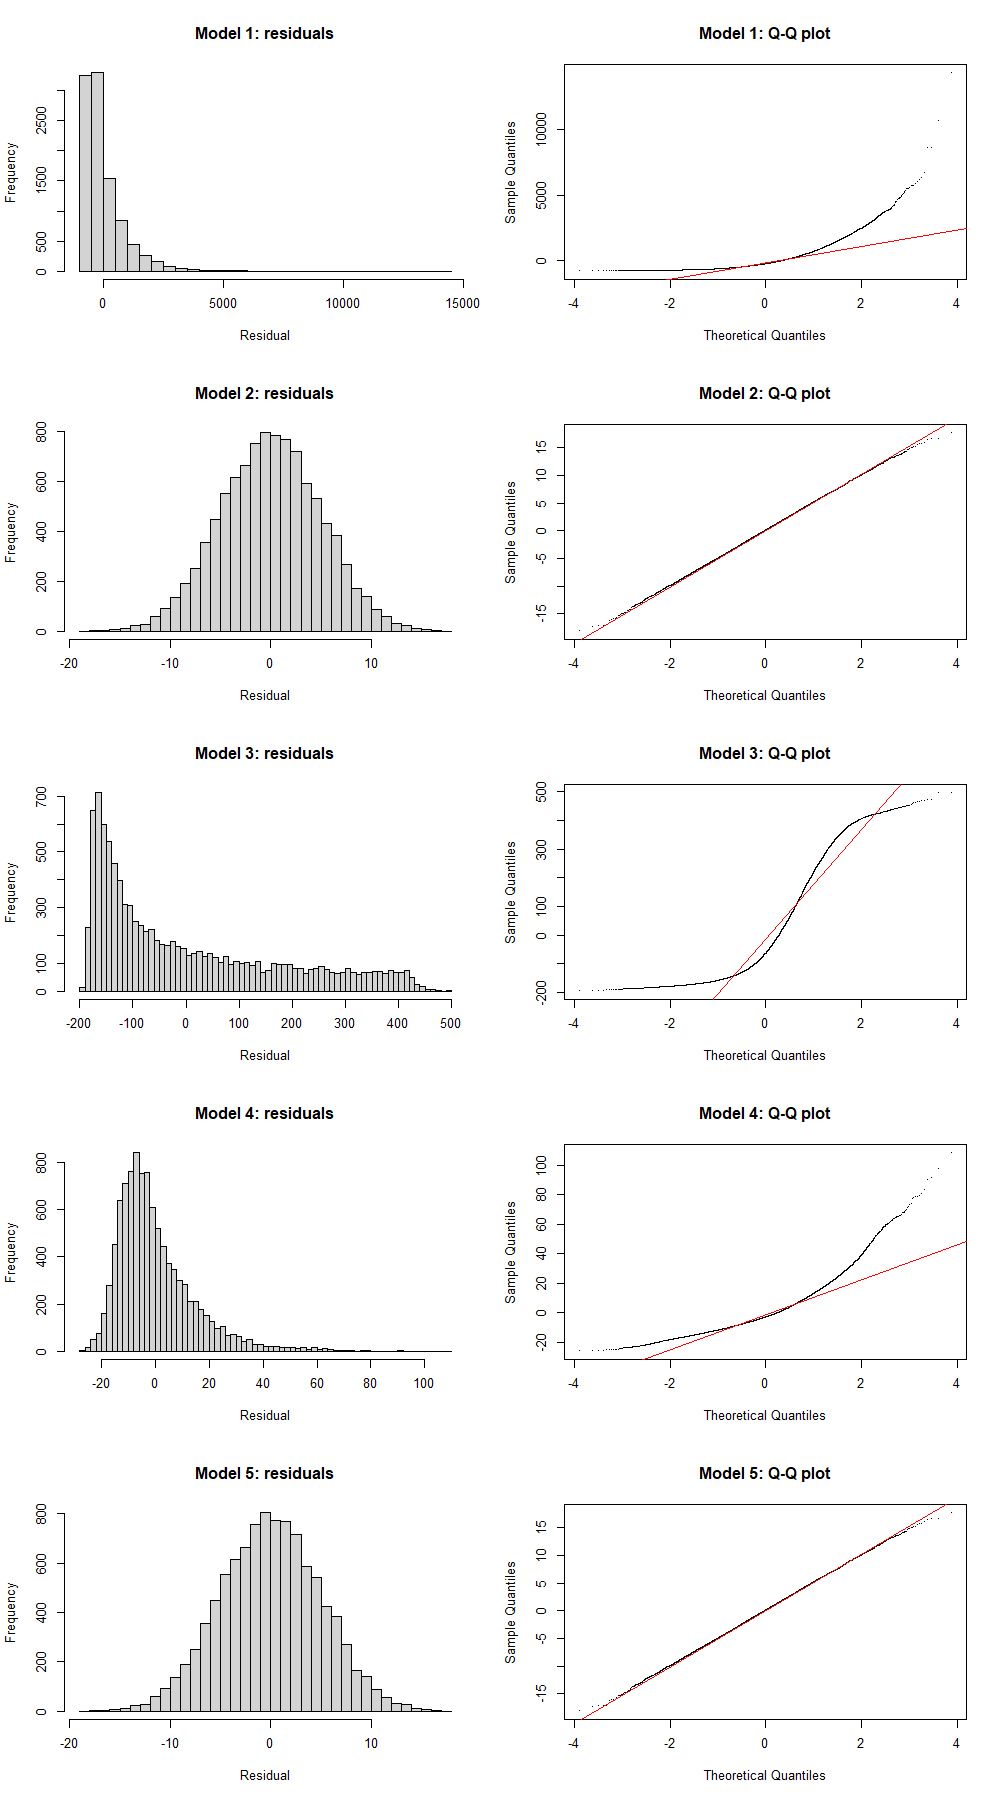
\includegraphics[width=0.72\textwidth]{fig5_residuals.png}
\caption{Residual histograms (left) and normal Q-Q plots (right) for the five candidate models.}
\label{fig:res}
\end{figure}

\subsection{Task 2.6: Selection of the best model}
Model~2 was chosen as the best model:
\begin{equation}
\hat{y}=4.4805\,x_4+1.2002\,x_1^3+0.8000\,x_3^4+120.02
\label{eq:best}
\end{equation}
The reasons are:
\begin{enumerate}
  \item \textbf{Information criteria:} it has the lowest AIC and the lowest BIC of the five models (\texttt{which.min()} returns 2 for both).
  \item \textbf{Residuals:} its residuals are symmetric, close to normal on the Q-Q plot, and pass the Shapiro--Wilk test. This is what we expect when the model structure is right and only the Gaussian measurement noise is left.
  \item \textbf{Parsimony:} Model~5 fits equally well but adds an $x_1^2$ term whose coefficient is almost zero ($-0.010$), so the term is not needed. According to \citet{burnham2002}, an AIC difference under 2 means that both models have support, so the decision rests on BIC, which favours Model~2 by 8.9 (strong evidence), and on choosing the simpler model. Model~2 is exactly Model~5 with $\theta_2=0$.
\end{enumerate}
The estimated coefficients are also very close to round numbers (0.8, 1.2, 4.48 and 120). This suggests that the simulated data were produced by a model with this exact structure, so Model~2 is very likely the ``true'' model.

\subsection{Task 2.7: Train/test validation and confidence intervals}
The data were split at random into 7000 training and 3000 test rows (\texttt{set.seed(123)}, Appendix~\ref{app:task2}, ``Task 2.7''). The same row indices were used for $\mathbf{X}$ and $\mathbf{y}$. Model~2 was refitted on the training rows only.

\textbf{1. Parameter estimates (training data).} $\hat\theta_1=4.4640$ ($x_4$), $\hat\theta_2=1.20015$ ($x_1^3$), $\hat\theta_3=0.800002$ ($x_3^4$) and $\hat\theta_{bias}=120.109$. These are almost identical to the full-data estimates, so the fit is stable.

\textbf{2. Test predictions.} On the 3000 unseen test rows the model reached an RMSE of 5.04\,W and $R^2=0.99996$. The RMSE is almost exactly the noise level estimated in Task~2.3 ($\hat\sigma\approx5.0$), so the model does not overfit: its test error is the noise floor. Figure~\ref{fig:predact} shows that all test predictions lie on the $y=x$ line.

\begin{figure}[H]
\centering
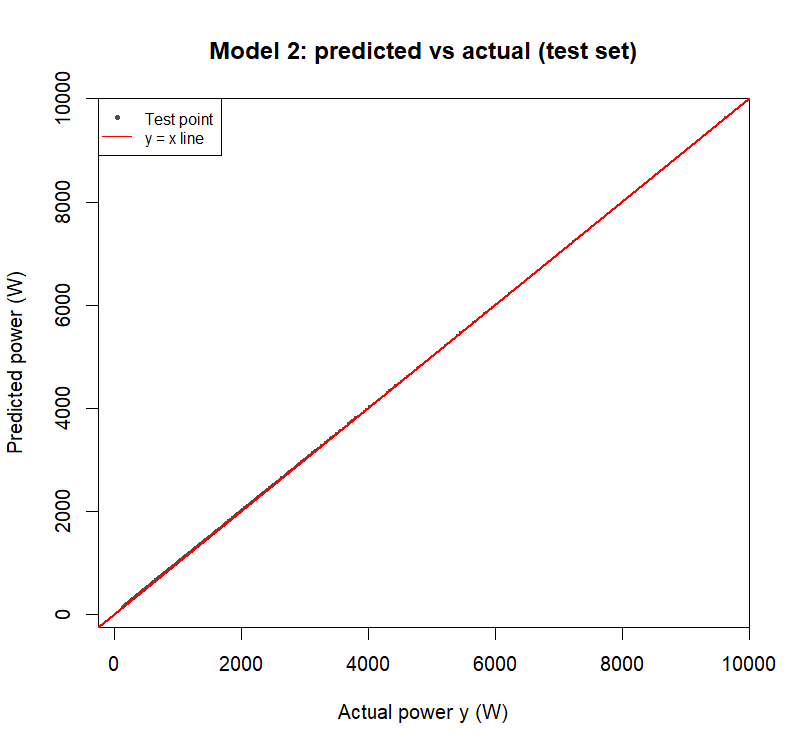
\includegraphics[width=0.55\textwidth]{fig6b_pred_vs_actual.png}
\caption{Predicted vs actual power for all 3000 test samples (Model~2 trained on 70\% of the data).}
\label{fig:predact}
\end{figure}

\textbf{3. 95\% confidence intervals.} The covariance of the estimates was computed as $\hat\sigma^2(\mathbf{X}_{tr}^T\mathbf{X}_{tr})^{-1}$ with $\hat\sigma^2=\text{RSS}_{tr}/(n_{tr}-k)$, and the critical value was $t_{0.975,6996}=1.960$. Figure~\ref{fig:ci} shows the first 40 test samples. In the top panel the predictions (red crosses) lie on top of the observed values (grey dots). The confidence intervals are very narrow, with a median width of only 0.38\,W (range 0.24--2.28\,W). On a scale of thousands of watts the error bars are shorter than the plotting symbols, so the bottom panel plots each point relative to its prediction, where the error bars (blue) can be seen.

\begin{figure}[H]
\centering
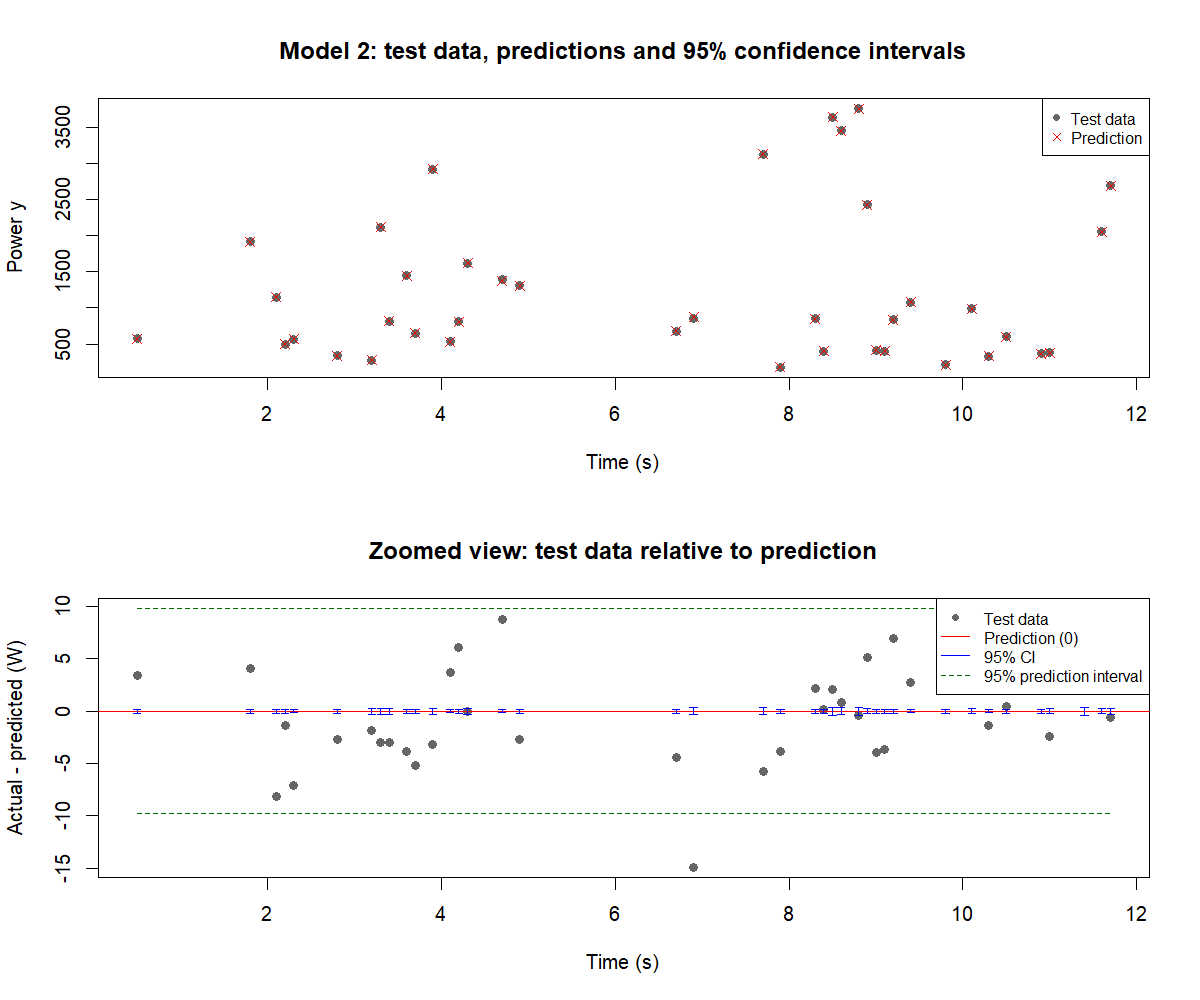
\includegraphics[width=0.95\textwidth]{fig6_confidence_intervals.png}
\caption{Model~2 predictions with 95\% confidence intervals for the first 40 test samples. Top: actual vs predicted power. Bottom: zoomed view of actual minus predicted, with 95\% confidence-interval error bars (blue) and 95\% prediction interval (dashed green).}
\label{fig:ci}
\end{figure}

It is important to tell the two kinds of interval apart. The confidence interval shows the uncertainty in the \emph{mean} prediction, which comes only from the uncertainty in $\hat{\boldsymbol\theta}$. With 7000 training samples this uncertainty is tiny, and only 3.7\% of the actual test values fall inside these intervals. That is expected, not a failure. The prediction interval adds the noise of a single new observation and is about $\pm9.8$\,W wide (total width 19.6\,W). It contains 94.6\% of the test values, very close to the nominal 95\%. This shows that the model and its error assumptions are well calibrated. The CI is widest for inputs far from the centre of the data, such as large $x_3$, because $x_3^4$ grows quickly there.
